\section{Minimization Problems with Constraints}
In applications, minimizers of our problem often have to satisfy additional conditions besides boundary conditions. These conditions are called constriants. The study of such minimization problems is the main subject in optimization theory.\\[11pt]

\begin{example}
\begin{itemize}
	\item[(a)] (Isovolumetric problem) Enclose given area with shortest possible circumference
	\[I(u):=\int_a^b{\sqrt{1+(u'(x))^2}\mathrm{d}x}.\]
	This we want to minimize subject to $\mathcal{J}(u):=\int_a^b{u(x)\mathrm{d}x}=A_0$, where $A_0\in\mathbb{R}$ is the given area. The minimization problem can be compactly written as
	\[\min\{I(u)\mid u(a)=u(b)=0\text{ and }\mathcal{J}(u)=A_0\}.\]
	Observe that in this example the constraint $\mathcal{J}$ is linear in $u$.
	\item[(b)] (Eigenvalue problem) Let $M\in\mathbb{R}^{n\times n}$ be symmetric and positive definite. We want to minimize
	\[I(u):=\frac{1}{2}(Mu)\cdot u\qquad\text{subject to}\qquad u\in\mathbb{R}^n\text{ and }\lvert u\rvert_2=2.\]
	Here, the constraint ``$\lvert u\rvert_2=2$'' is nonlinear. The Problem can be written compactly as
	\[\min\{I(u)\mid\mathcal{J}(u)=1\},\]
	where $\mathcal{J}(u):=\frac{1}{2}\lvert u\rvert_2^2$. Later we will see that minimizers $u_*\in\mathbb{R}^n$ necessarily have to satisfy $DI(u_*)=\lambda_* D\mathcal{J}(u_*)$ for some $\lambda_*\in\mathbb{R}$. But this means $Mu_*=\lambda_*u_*$, i.e., $u_*$ is an eigenvector for the eigenvalue $\lambda_*$. In particular we have $I(u_*)=\frac{1}{2}(Mu_*)\cdot u_*=\frac{\lambda_*}{2}\lvert u_*\rvert_2^2=\lambda_*$.\\

	In infinite-dimensional setting, we can equivalently ask to minimize $\min\{I(u)\mid\mathcal{J}(u)=1\}$ where
	\[I(u)=\int_\Omega{\lvert\nabla u(x)\rvert^2\mathrm{d}x}\quad\text{and}\quad\mathcal{J}(u)=\int_\Omega{(u(x))^2\mathrm{d}x}\]
	for $u\in H_0^1(\Omega)$. A minimizer $u_*$ then has to satisfy
	\[\int_\Omega{\nabla u_*(x)\cdot\nabla v(x)\mathrm{d}x}=\lambda_*\int_\Omega{u_*(x)v(x)\mathrm{d}x}\]
	for all $v\in H_0^1(\Omega)$. So $\lambda_*$ is an eigenvalue of the Laplacian $-\Delta$ on $H_0^1(\Omega)$, so $-\Delta u_*=\lambda_*u_*$, $u_*=0$ on $\partial\Omega$, holds in the weak sense.
	\item[(c)] (Obstacle problem) Let $u:\Omega\longrightarrow\mathbb{R}$ describe a membrane stretched over an obstacle which is denoted by $\psi:\Omega\longrightarrow\mathbb{R}$.\\

	\begin{figure}[ht]
		\centering
		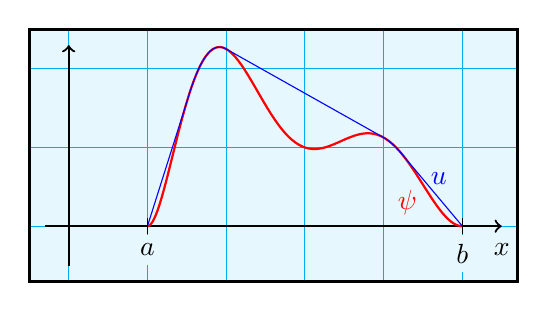
\begin{tikzpicture}
			\fill[cyan!10] (-0.5, -0.7) rectangle (5.7, 2.5);
			\draw[cyan] (-0.5, -0.7) grid (5.7, 2.5);
			\draw[thick, ->] (-0.3, 0) -- (5.5, 0);
			\draw[thick, ->] (0, -0.5) -- (0, 2.3);

			\draw[thick, red] plot[smooth, domain=-2:2, samples=200] ({\x+3}, {(3-\x)*((\x)^6-15/2*(\x)^4+12*(\x)^2+8)/24});
			\draw[blue] (1, 0) -- (1.522, 1.648);
			\draw[blue] plot[smooth, domain=-1.48:-1] ({\x+3}, {(3-\x)*((\x)^6-15/2*(\x)^4+12*(\x)^2+8)/24});
			\draw[blue] (2, 2.25) -- (4, 1.125);
			\draw[blue] plot[smooth, domain=1:1.23] ({\x+3}, {(3-\x)*((\x)^6-15/2*(\x)^4+12*(\x)^2+8)/24});
			\draw[blue] (4.228, 0.920) -- (5, 0);

			\draw[thin] (1, 0.1) -- (1, -0.1) node[below, fill=cyan!10] {$a$};
			\draw[thin] (5, 0.1) -- (5, -0.1) node[below, fill=cyan!10] {$b$};
			\node at (5.5, -0.3) {$x$};
			\node[red] at (4.3, 0.3) {$\psi$};
			\node[blue] at (4.7, 0.6) {$u$};

			\draw[very thick] (-0.5, -0.7) rectangle (5.7, 2.5);
		\end{tikzpicture}
		\caption{Illustration of Obstacle problem.}
	\end{figure}

	Then minimize the functional $I(u)=\int_\Omega{\sqrt{1+\lvert\nabla u(x)\rvert^2}\mathrm{d}x}$ subject to $u(x)\geq\psi(x)$ for almost every $x\in\Omega$, and $u\vert_{\partial\Omega}=0$.\\

	Caveat: $f(A)=\sqrt{1+\lvert A\rvert^2}$ grows linear. Hence, coercivity holds only on $W_0^{1,1}(\Omega)$ which is a bad space as it is not reflexive. But there is a way out by simplification the model via Taylor expansion
	\[f(A)=f(0)+\partial_Af(0)\cdot A+\frac{1}{2}\partial_A^2f(0)A\cdot A+o(\lvert A\rvert^2).\]
	So for $\lvert A\rvert$ small it holds $f(A)=1+\frac{1}{2}\lvert A\rvert^2$. So we consider
	\[\widetilde{I}(u)=\int_\Omega{\left(1+\frac{1}{2}\lvert\nabla u(x)\rvert^2\right)\mathrm{d}x},\]
	which is coercive on $H_0^1(\Omega)$, subject to $u(x)\geq\psi(x)$ for almost every $x\in\Omega$.\\[11pt]
\end{itemize}
\end{example}

\begin{theorem}
Let $X$ be a reflexive Banach space, $M\subset X$ non-empty, weakly sequentially closed, $I:M\longrightarrow\mathbb{R}_\infty$ coercive on $M$ and weakly sequentially lower semicontinuous on $X$. Then there exists $u_*\in M$ such that
\[I(u_*)=\inf_{u\in M}{I(u)}.\]
Note that the constraint is encoded in the subset $M$.\\
\end{theorem}

\begin{proof}
The proof follows the same strategy as \hyperlink{theorem_3_1_14}{Theorem 3.1.14}.\hfill$\blacksquare$\\[11pt]
\end{proof}


In \hyperlink{examples_3_6_1}{Examples 3.6.1}, we had the sets
\begin{itemize}
	\item[(a)] $M=\{u\in H^1(\Omega)\mid u(a)=u(b)=0,\int_a^b{u(x)\mathrm{d}x}=A_0\}$,
	\item[(b)] $M=\{u\in H_0^1(\Omega)\mid\lVert u\rVert_{L^2(\Omega)}=1\}$,
	\item[(c)] $M=\{u\in H_0^1(\Omega)\mid u(x)\geq\psi(x)\text{ for almost every }x\in\Omega\}$.
\end{itemize}
Sometimes, like in (c) if e.g. $\psi\vert_{\partial\Omega}>0$, it is not clear that $M$ is non-empty. But mostly the crucial question is: When is $M\subset X$ weakly sequentially closed?\\[11pt]

\begin{example}
\begin{itemize}
	\item[(a)] If $M$ is convex, then Mazur's lemma tells us that $M$ is weakly sequentially closed if it is strongly closed.
	\item[(b)] But $M$ does not need to be convex for weak sequential closedness. As an example, consider a set-valued map $\Phi:\Omega\longrightarrow\mathcal{P}(\mathbb{R})$ with $\mathcal{P}(\mathbb{R})$ being the power set of $\mathbb{R}$, satisfying $\Phi(x)\subset\mathbb{R}$ closed, non-empty for all $x\in\Omega$. Then, for $p\geq1$ define
	\[M=\{u\in W^{1,p}(\Omega)\mid u(x)\in\Phi(x)\text{ for almost every }x\in\Omega\}.\]
	First we should mention that it can happen that $M$ is non-empty.

	\begin{figure}[ht]
		\centering
		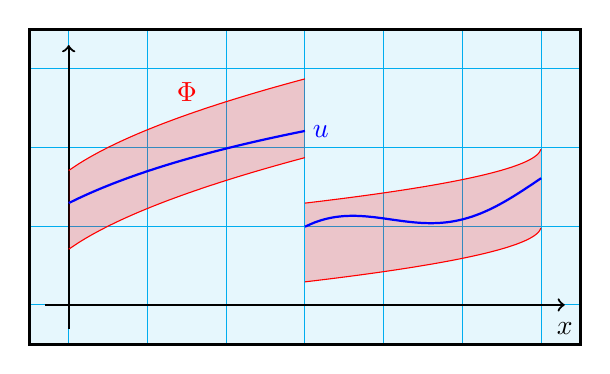
\begin{tikzpicture}
			\fill[cyan!10] (-0.5, -0.5) rectangle (6.5, 3.5);
			\draw[cyan] (-0.5, -0.5) grid (6.5, 3.5);
			\draw[thick, ->] (-0.3, 0) -- (6.3, 0);
			\node at (6.3, -0.3) {$x$};
			\draw[thick, ->] (0, -0.3) -- (0, 3.3);

			\fill[red, opacity=0.2] plot[smooth, domain=0:3] (\x, {sqrt(\x+0.5)}) -- (3, 2.871) plot[smooth, domain=3:0] (\x, {1+sqrt(\x+0.5)}) -- (0, 0.707);
			\fill[red, opacity=0.2] plot[smooth, domain=3:6, samples=200] (\x, {2-sqrt(1-\x/6)}) -- (6, 1) plot[smooth, domain=6:3, samples=200] (\x, {1-sqrt(1-\x/6)}) -- (3, 1.293);
			\draw[red] plot[smooth, domain=0:3] (\x, {sqrt(\x+0.5)});
			\draw[red] plot[smooth, domain=0:3] (\x, {1+sqrt(\x+0.5)});
			\draw[red] plot[smooth, domain=3:6, samples=200] (\x, {1-sqrt(1-\x/6)});
			\draw[red] plot[smooth, domain=3:6, samples=200] (\x, {2-sqrt(1-\x/6)});

			\draw[thick, blue] plot[smooth, domain=0:3] (\x, {0.6+ln(\x+2)});
			\draw[thick, blue] plot[smooth, domain=3:6] (\x, {ln(\x-1)+0.3*cos((\x-3)*90)});

			\node[red] at (1.5, 2.7) {$\Phi$};
			\node[blue] at (3.2, 2.2) {$u$};
			\draw[very thick] (-0.5, -0.5) rectangle (6.5, 3.5);
		\end{tikzpicture}
		\caption{$\Phi$ with a sort of jump.}
		\label{fig:example_3_6_3_empty}
	\end{figure}

	\begin{figure}[ht]
		\centering
		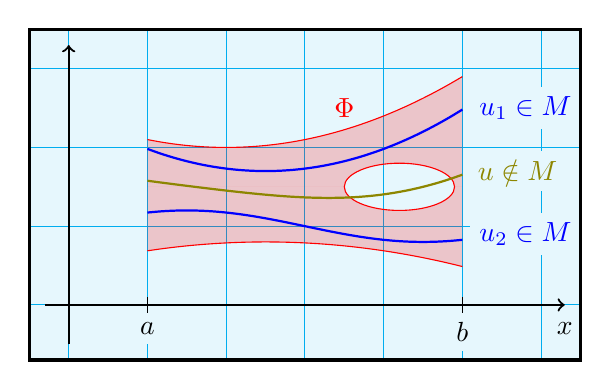
\begin{tikzpicture}
			\fill[cyan!10] (-0.5, -0.7) rectangle (6.5, 3.5);
			\draw[cyan] (-0.5, -0.7) grid (6.5, 3.5);
			\draw[thick, ->] (-0.3, 0) -- (6.3, 0);
			\node at (6.3, -0.3) {$x$};
			\draw[thick, ->] (0, -0.5) -- (0, 3.3);
			\draw[thin] (1, 0.1) -- (1, -0.1) node[below, fill=cyan!10] {$a$};
			\draw[thin] (5, 0.1) -- (5, -0.1) node[below, fill=cyan!10] {$b$};

			\fill[red, opacity=0.2] plot[smooth, domain=1:5] (\x, {2+(\x-2)^2/10}) -- (5, 1.5) -- (4.9, 1.5) arc (0:180:0.7 and 0.3) -- (1, 1.5) -- (1, 2.1);
			\fill[red, opacity=0.2] plot[smooth, domain=1:5] (\x, {0.8-(\x-2.5)^2/20}) -- (5, 1.5) -- (4.9, 1.5) arc (360:180:0.7 and 0.3) -- (1, 1.5) -- (1, 0.9125);
			\draw[red] plot[smooth, domain=1:5] (\x, {2+(\x-2)^2/10});
			\draw[red] plot[smooth, domain=1:5] (\x, {0.8-(\x-2.5)^2/20});
			\draw[red] (4.2, 1.5) ellipse (0.7 and 0.3);

			\draw[thick, blue] plot[smooth, domain=1:5] (\x, {1.7+(\x-2.5)^2/8});
			\draw[thick, blue] plot[smooth, domain=1:5] (\x, {1+0.2*sin(\x*60)});
			\draw[thick, olive] plot[smooth, domain=1:5] (\x, {1.35+(\x-2.5)^2/16+sin(\x*60)/10});

			\node[red] at (3.5, 2.5) {$\Phi$};
			\node[blue, fill=cyan!10] at (5.8, 2.5) {$u_1\in M$};
			\node[olive, fill=cyan!10] at (5.7, 1.7) {$u\notin M$};
			\node[blue, fill=cyan!10] at (5.8, 0.9) {$u_2\in M$};
			\draw[very thick] (-0.5, -0.7) rectangle (6.5, 3.5);
		\end{tikzpicture}
		\caption{$\Phi(x)$ not connected for all $x\in[a,b]$.}
		\label{fig:example_3_6_3_not_connected}
	\end{figure}

	For example, for a $\Phi$ such as in \hyperref[fig:example_3_6_3_empty]{Figure III.11}, $M$ is empty because any $u$ with $u(x)\in\Phi(x)$ has a jump. Moreover, if e.g. $\Phi(x)$ is not connected for all $x$ (illustrated in \hyperref[fig:example_3_6_3_not_connected]{Figure III.12}), then $M$ is not convex.\\

	But $M$ is weakly sequentially closed as a subset of $W^{1,p}(\Omega)$. Indeed, let $(u_n)_{n\in\mathbb{N}}\subset M$, $u\in W^{1,p}(\Omega)$ such that $u_n\rightharpoonup u$ in $W^{1,p}(\Omega)$ for $n\to\infty$. We need $u\in M$. By Rellich's compact theorem we have $u_n\to u$ in $L^p(\Omega)$. So there exists a subsequence $(u_{n_k})_{k\in\mathbb{N}}\subset(u_n)_{n\in\mathbb{N}}$ such that $u_{n_k}(x)\to u(x)$ for $k\to\infty$ and almost all $x\in\Omega$. Since $\Phi(x)\subset\mathbb{R}$ is closed, we therefore have $u(x)\in\Phi(x)$ for almost all $x\in\Omega$. Thus, $u\in M$.\\[11pt]
\end{itemize}
\end{example}

\begin{corollary}
(\hyperlink{examples_3_6_1}{Examples 3.6.1 (c)}, Obstacle problem)\\
Let $\Omega\subset\mathbb{R}^d$ be bounded, open with Lipschitz boundary. For $\psi\in H_0^1(\Omega)$ define
\[M_\psi:=\{u\in H_0^1(\Omega)\mid u\geq\psi\text{ almost everywhere in }\Omega\}.\]
Set $\Phi(x)=[\psi(x),+\infty)$ which is closed in $\mathbb{R}$. As $\psi\in M_\psi$, we have $M_\psi\ne\emptyset$.\\

Hence $M_\psi$ is weakly sequentially closed. \hyperlink{theorem_3_6_2}{Theorem 3.6.2} therefore yields a minimizer $u_*\in M_\psi$ of
\[\widetilde{I}(u)=\int_\Omega{1+\frac{1}{2}\lvert\nabla u(x)\rvert^2\mathrm{d}x}\]\\[11pt]
\end{corollary}

\begin{example}
Consider $X=W^{1,p}(\Omega)$, $p\in(1,\infty)$, $\mathcal{J}(u)=\lVert u\rVert_{L^r(\Omega)}^r$ and $M=\{u\in X\mid\mathcal{J}(u)=1\}$. We ask when $M$ is weakly sequentially closed. The idea is to use Rellich's compact embedding, so we need $1\geq\frac{1}{r}\geq\frac{d-p}{dp}$ in order to have the compact embedding $W^{1,p}(\Omega)\clonghookrightarrow L^r(\Omega)$. Hence, $u_n\rightharpoonup u$ in $W^{1,p}(\Omega)$ yields $u_n\to u$ in $L^r(\Omega)$, and then $\mathcal{J}(u)=\lim_{n\to\infty}{\mathcal{J}(u_n)}=1$.
\end{example}

Next we want to treat the question whether we can characterize minimizers $u_*$ via suitable Euler-Lagrange equations. To answer this question, we restrict our discussion to equality constraints, i.e. of the form $\mathcal{J}(u)=a$ for some $a\in\mathbb{R}$. For applications this is really restrictive and usually inequality constraints are of more interest. The obstacle problem for example is no equality constraint. Inequality constraints are related to so-called (KKT) conditions (``Karush-Kuhn-Tucker''). This is program in optimization theory.\\

In the following we will write for Banach spaces $X,Y$
\[C^1(X,Y):=\{\mathcal{J}:X\longrightarrow Y\mid\mathcal{J}\text{ is Fr\'echet differentiable}\},\]
that means $\mathcal{J}$ is G\^ateaux differentiable and $D\mathcal{J}:X\longrightarrow\Lin{X}{Y}$ is continuous, where $\Lin{X}{Y}$ denotes the space of all continuous, linear maps from $X$ to $Y$. The notion goes back to \textsc{Maurice Fr\'echet} (* 1878; $\dagger$ 1973). He was a student of Hadamard.\\

\begin{theorem}[Lagrange multipliers]
Let $X$ be a reflexive Banach space, $I,\mathcal{J}\in C^1(X;\mathbb{R})$. Put $M_\alpha:=\{u\in X\mid\mathcal{J}(u)=\alpha\}$ for $\alpha\in\mathbb{R}$ and suppose $M_\alpha\ne\emptyset$. Further assume that
\begin{itemize}
	\item[(a)] $I$ is weakly sequentially lower semicontinuous on $X$;
	\item[(b)] $\mathcal{J}$ is weakly sequentially continuous on $X$;
	\item[(c)] $I:M_\alpha\longrightarrow\mathbb{R}$ is coercive.
\end{itemize}
Then
\begin{itemize}
	\item[(i)] $I:M_\alpha\longrightarrow\mathbb{R}$ has a minimizer $u_*\in M_\alpha$.
	\item[(ii)] If in addition $D\mathcal{J}(u_*)\ne0$ then there exists $\lambda_*\in\mathbb{R}$, a so-called \textit{Lagrange multiplier}, such that $DI(u_*)=\lambda_*D\mathcal{J}(u_*)\in X'$.\\
\end{itemize}
\end{theorem}

\begin{remark}
\begin{itemize}
	\item[(a)] Let's consider a more specific setting. Let $X=W_0^{1,p}(\Omega;\mathbb{R}^m)$ for $p\in(1,\infty)$, and let $f:\Omega\times\mathbb{R}^m\times\mathbb{R}^{m\times d}\longrightarrow\mathbb{R}$, $h:\Omega\times\mathbb{R}^m\longrightarrow\mathbb{R}$ be such that
	\[I(u):=\int_\Omega{f(x,u(x),\nabla u(x))\mathrm{d}x}\quad\text{and}\quad\mathcal{J}(u):=\int_\Omega{h(x,u(x))\mathrm{d}x}\]
	satisfy the assumptions of \hyperlink{theorem_3_6_6}{Theorem 3.6.6}. Then the weak Euler-Lagrange equations with constraint given by $\mathcal{J}$ is
	\[\int_\Omega{\partial_Af(\cdot,u_*,\nabla u_*):\nabla v+\partial_uf(\cdot,u_*,\nabla u_*)\cdot v\mathrm{d}x}=\lambda_*\int_\Omega{\partial_uh(\cdot,u_*)\cdot v\mathrm{d}x}\]
	for all $v\in W_0^{1,p}(\Omega;\mathbb{R}^m)$.
	\item[(b)] If $\mathcal{J}:X\longrightarrow Y$, i.e. $\mathcal{J}$ maps into a general (possibly infinite-dimensional) Banach space, and $M_{y_0}=\{u\in X\mid\mathcal{J}(u)=y_0\}$ for some $y_0\in Y$, then there is a Theorem by Ljusternik that gives $\lambda_*\in Y'$ so that the Euler-Lagrange equations are
	\[DI(u_*)[v]=\lambda_*(\underbrace{D\mathcal{J}(u_*)[v]}_{\in Y})\]
	for all $v\in X$. See \cite[Chapter 4, 4.2 Ljusternik's Theorems]{blanchard_bruening}.\\
\end{itemize}
\end{remark}

For the proof of \hyperlink{theorem_3_6_6}{Theorem 3.6.6} we need the following preliminary result.\\

\begin{theorem}[Implicit Function Theorem]
Let $X,Y,Z$ be Banach spaces, $F:X\times Y\longrightarrow Z$ a $C^1$-function. Let $(x_0,y_0)\in X\times Y$ such that $F(x_0,y_0)=0\in Z$ and $(D_yF(x_0,y_0))^{-1}\in\operatorname{Lin}(Z,Y)$ exists. Then, there exist $\varepsilon>0$, $\Phi_0\in C^1(B_\varepsilon(x_0),Y)$ (with $B_\varepsilon(x_0)=\{x\in X\mid \lVert x-x_0\rVert_X<\varepsilon\}$) such that
\begin{itemize}
	\item[(i)] $\Phi_0(x_0)=y_0$,
	\item[(ii)] $F(x,\Phi_0(x))=0$ for all $x\in B_\varepsilon(x_0)$,
	\item[(iii)] From $F(x,y)=0$ and $\lVert x-x_0\rVert+\lVert y-y_0\rVert<\varepsilon$ it follows $\Phi_0(x)=y$.\\
\end{itemize}
\end{theorem}

\begin{proof}
The proof can be found in \cite[Kapitel III, III.5 Differentiation nichtlinearer Abbildungen, Satz III.5.4 (e)]{dirk_werner}.\\[11pt]

\textit{Proof of \hyperlink{theorem_3_6_6}{Theorem 3.6.6}:}\\
First note that the existence of a minimizer $u_*\in M_\alpha$ follows from weak closedness of the set $M_\alpha\subset X$ and \hyperlink{theorem_3_6_2}{Theorem 3.6.2}. The proof of assertion (ii) is divided into three steps.\\

\textit{Step 1:}
\begin{itemize}
	\item[] We describe $M_\alpha$ locally around $u_*\in M_\alpha$ over tangent space. The tangent space of $M_\alpha$ in $u_*$ is
	\[V_{u_*}=\{v\in X\mid D\mathcal{J}(u_*)[v]=0\},\]
	and $V_{u_*}$ is a subspace of $X$ because $D\mathcal{J}(u_*)$ is linear. By assumption $D\mathcal{J}(u_*)\ne0$, there exists $v_1\in X$ such that $D\mathcal{J}(u_*)[v_1]=1$. Define the function
	\[F:V_{u_*}\times\mathbb{R}\longrightarrow\mathbb{R},\qquad F(v,\delta):=\mathcal{J}(u_*+v+\delta v_1)-\alpha.\]
	We know
	\begin{itemize}
		\item[(1)] $F(0,0)=0$ since $u_*\in M_\alpha$,
		\item[(2)] $F\in C^1(V_{u_*}\times\mathbb{R})$ since $\mathcal{J}$ is a $C^1$-function, and
		\item[(3)] $\partial_\delta F(0,0)=D\mathcal{J}(u_*)[v_1]=1$.
	\end{itemize}

	\begin{figure}[ht]
		\centering
		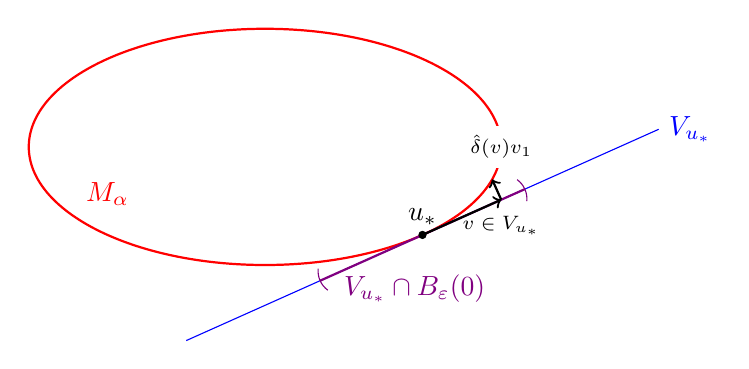
\begin{tikzpicture}
			\draw[thick, red] ellipse (3 and 1.5);
			\draw[blue] (-1, -2.4597) -- (5, 0.2236);

			\draw[thick, violet] (0.7, -1.6994) -- (3.3, -0.5366);
			\draw[violet] (3.3, -0.5366) arc (24.1:54.1:0.3);
			\draw[violet] (3.3, -0.5366) arc (24.1:-5.9:0.3);
			\draw[violet] (0.7, -1.6994) arc (204.1:234.1:0.3);
			\draw[violet] (0.7, -1.6994) arc (204.1:174.1:0.3);

			\draw[thick, ->] (2, -1.118) -- (3, -0.6708);
			\draw[thick, ->] (3, -0.6708) -- (2.8844, -0.4124);

			\node[red] at (-2, -0.6) {$M_\alpha$};
			\node[blue] at (5.4, 0.2236) {$V_{u_*}$};
			\node at (3, -1) {\scriptsize$v\in V_{u_*}$};
			\node[fill=white] at (3, 0) {\scriptsize$\hat{\delta}(v)v_1$};
			\node[violet] at (1.9, -1.8) {$V_{u_*}\cap B_\varepsilon(0)$};
			\fill (2, -1.118) circle (1.5pt) node[above] {$u_*$};
		\end{tikzpicture}
		\caption{Illustration of tangent space $V_{u_*}$ and function $\hat{\delta}$.}
	\end{figure}

	Hence, the implicit function theorem, i.e. \hyperlink{theorem_3_6_8}{Theorem 3.6.8}, gives $\varepsilon>0$ and a mapping $\hat{\delta}\in C^1(V_{u_*}\cap B_\varepsilon(0);\mathbb{R})$ with $\hat{\delta}(0)=0$ and $F(v,\hat{\delta}(v))=0$ for all $v\in V_{u_*}\cap B_\varepsilon(0)$ (here, $B_\varepsilon(0)=\{x\in X\mid\lVert x\rVert_X<\varepsilon\}$). The last property means $\mathcal{J}(u_*+v+\hat{\delta}(v)v_1)=\alpha$ for all $v\in V_{u_*}\cap B_\varepsilon(0)$, so that
	\begin{align}\label{eq:mcov_formula_3_4}
		\{u_*+v+\hat{\delta}(v)v_1\mid v\in V_{u_*}\cap B_\varepsilon(0)\}\subseteq M_\alpha.
	\end{align}\\
\end{itemize}

\textit{Step 2:} We show that $DI(u_*)[w]=0$ for all $w\in V_{u_*}$.
\begin{itemize}
	\item[] Define $\widetilde{I}(v):=I(u_*+v+\hat{\delta}(v)v_1)$ for $v\in V_{u_*}\cap B_\varepsilon(0)$. As $u_*$ minimizes $I$, we get $\widetilde{I}(0)\leq\widetilde{I}(v)$ for all $v\in V_{u_*}\cap B_\varepsilon(0)$ by \eqref{eq:mcov_formula_3_4}. Thus,
	\[\lim_{h\searrow0}{\frac{\widetilde{I}(hw)-\widetilde{I}(0)}{h}}\geq0\]
	for all $w\in V_{u_*}$, and hence $D\widetilde{I}(0)[w]\geq0$. By replacing $w$ by $-w$ (remind $V_{u_*}$ is a linear space) we even get $D\widetilde{I}(0)[w]=0$ for all $w\in V_{u_*}$. Via chain rule this means
	\begin{align}\label{eq:mcov_formula_3_5}
		D\widetilde{I}(0)=DI(u_*)[w+D\hat{\delta}(0)[w]v_1]=0
	\end{align}
	for all $w\in V_{u_*}$. We claim $D\hat{\delta}(0)[w]=0$ for all $w\in V_{u_*}$. We know $G(v):=F(v,\hat{\delta}(v))=0$ for all $v\in V_{u_*}\cap B_\varepsilon(0)$. Fix $w\in V_{u_*}$. Then
	\[0=D_vG(v)[w]=D_vF(v,\hat{\delta}(v))[w]+D_\delta F(v,\hat{\delta}(v))[D\hat{\delta}(v)[w]].\]
	Using the definition of $F$ in terms of $\mathcal{J}$ we get
	\[0=D\mathcal{J}(u_*+v+\hat{\delta}(v)v_1)[w]+D\mathcal{J}(u_*+v+\hat{\delta}(v)v_1)[v_1]D\hat{\delta}(v)[w].\]
	Thus, for $v=0$ we get
	\[0=\underbrace{D\mathcal{J}(u_*)[w]}_{=0\text{ as }w\in V_{u_*}}+\underbrace{D\mathcal{J}(u_*)[v_1]}_{=1\text{ choice of }v_1}D\hat{\delta}(0)[w],\]
	i.e., $D\hat{\delta}(0)[w]=0$ as claimed. Therefore, $DI(u_*)[w]=0$ for all $w\in V_{u_*}$ by \eqref{eq:mcov_formula_3_5}.\newpage
\end{itemize}

\textit{Step 3:}
\begin{itemize}
	\item[] Write $X$ as the direct sum of $V_{u_*}$ and $\operatorname{span}\{v_1\}$, so $X=V_{u_*}\oplus\operatorname{span}\{v_1\}$. Indeed, if $w\in X$ is given, write $D\mathcal{J}(u_*)[w]=\beta_w$ and $v=w-\beta_wv_1$. We check
	\[D\mathcal{J}(u_*)[v]=D\mathcal{J}(u_*)[w]-\beta_wD\mathcal{J}(u_*)[v_1]=\beta_w-\beta_w\cdot 1=0.\]
	Therefore, $v\in V_{u_*}$. Moreover, for $w=v+\beta_wv_1$ we have
	\[DI(u_*)[w]=\underbrace{DI(u_*)[v]}_{=0\text{ by step 2.}}+\beta_w\underbrace{DI(u_*)[v_1]}_{=:\lambda_*}=\beta_w\lambda_*=\lambda_*D\mathcal{J}(u_*)[w].\]
\end{itemize}
\end{proof}

\begin{example}[Eigenvalue of Laplacian]
Let $\Omega\subset\mathbb{R}^d$ be an open, bounded domain with Lipschitz boundary. Consider $X=H_0^1(\Omega)$ and
\[I(u)=\int_\Omega{\lvert\nabla u(x)\rvert^2\mathrm{d}x},\qquad\mathcal{J}(u)=\int_\Omega{\lvert u(x)\rvert^2\mathrm{d}x}.\]
\textit{Definition:} We call $\lambda\in\mathbb{C}$ an \textit{eigenvalue of Laplacian $(-\Delta)$ on $H_0^1(\Omega)$} if $u_\lambda\in H_0^1(\Omega)\setminus\{0\}$ exists such that for all $v\in H_0^1(\Omega)$
\[\int_\Omega{\nabla u_\lambda(x)\cdot\nabla v(x)\mathrm{d}x}=\lambda\int_\Omega{u_\lambda(x)v(x)\mathrm{d}x}.\]
This is the weak formulation of the partial differential equation
\[\left\{\begin{array}{rl}
	-\Delta u_\lambda=\lambda u_\lambda&\text{in }\Omega,\\
	u=0&\text{on }\partial\Omega.
\end{array}\right.\]
In this case, $u_\lambda$ is called an \textit{eigenfunction}.\\

We claim:
\begin{itemize}
	\item[(a)] All eigenvalues are real and positive.
	\item[(b)] The smallest eigenvalue $\lambda_{\text{min}}>0$ exists and is given by
	\[\lambda_\text{min}=\min_{\substack{u\in H_0^1(\Omega)\\u\ne0}}{\frac{I(u)}{\mathcal{J}(u)}}=\min_{\substack{u\in H_0^1(\Omega)\\\mathcal{J}(u)=1}}{I(u)},\]
	and all minimizers are eigenfunctions.\\
\end{itemize}

We want to prove this.
\begin{itemize}
	\item[(a)] Set $v=u_\lambda$ in the weak formulation to obtain $\lambda\in\mathbb{R}$ and $\lambda>0$.
	\item[(b)] Consider
	\[\min\{I(u)\mid u\in H_0^1(\Omega)\text{ and }\mathcal{J}(u)=1\}.\]
	Part (i) of \hyperlink{theorem_3_6_6}{Theorem 3.6.6} is applicable on $M_1=\{u\in H_0^1(\Omega)\mid\mathcal{J}(u)=1\}$ because this is weakly sequentially closed as $H_0^1(\Omega)\clonghookrightarrow L^2(\Omega)$. So there exists $u_*\in M_1$ so that
	\begin{align*}
		I(u_*)&=\min_{u\in M_1}{\int_\Omega{\lvert\nabla u(x)\rvert^2\mathrm{d}x}}=\min_{\substack{\tilde{u}\in H_0^1(\Omega)\\\tilde{u}\ne0}}{\int_\Omega{\left\lvert\nabla\frac{\tilde{u}(x)}{\lVert\tilde{u}\rVert_{L^2(\Omega)}}\right\rvert^2\mathrm{d}x}}\\
		&=\min_{\substack{\tilde{u}\in H_0^1(\Omega)\\\tilde{u}\ne0}}{\frac{\int_\Omega{\lvert\nabla\tilde{u}(x)\rvert^2\mathrm{d}x}}{\int_\Omega{\lvert\tilde{u}(x)\rvert^2\mathrm{d}x}}}=\min_{\substack{\tilde{u}\in H_0^1(\Omega)\\\tilde{u}\ne0}}{\frac{I(\tilde{u})}{\mathcal{J}(\tilde{u})}}.
	\end{align*}
	We have $D\mathcal{J}(u_*)[w]=2\int_\Omega{u_*(x)w(x)\mathrm{d}x}$ for all $w\in H_0^1(\Omega)$. For $w=u_*$ it follows $D\mathcal{J}(u_*)[u_*]=2\lVert u_*\rVert_{L^2(\Omega)}^2=2\ne0$. Thus, assertion (ii) of \hyperlink{theorem_3_6_6}{Theorem 3.6.6} gives existence of $\lambda_*\in\mathbb{R}$ such that $DI(u_*)=\lambda_*D\mathcal{J}(u_*)$. This means explicitly that
	\[\int_\Omega{\nabla u_*(x)\cdot\nabla v(x)\mathrm{d}x}=\lambda_*\int_\Omega{u_*(x)v(x)\mathrm{d}x}\]
	for all $v\in H_0^1(\Omega)$ (after division by 2). So $u_*$ is indeed an eigenfunction for the eigenvalue $\lambda_*$, and we see, if we set $v=u_*$ again, that $\lambda_*$ is the minimum, i.e.
	\[\min_{\substack{u\in H_0^1(\Omega)\\u\ne0}}{\frac{I(u)}{\mathcal{J}(u)}}=I(u_*)=\int_\Omega{\lvert\nabla u_*(x)\rvert^2\mathrm{d}x}=\lambda_*\int_\Omega{\lvert u_*(x)\rvert^2\mathrm{d}x}=\lambda_*.\]
	It remains to show that $\lambda_*$ is the smallest eigenvalue. Suppose $\tilde{\lambda}>0$ is an eigenvalue with $\lambda_*>\tilde{\lambda}$ and some eigenfunction $\tilde{u}\in H_0^1(\Omega)\setminus\{0\}$. Then in particular
	\[\int_\Omega{\lvert\nabla\tilde{u}(x)\rvert^2\mathrm{d}x}=\tilde{\lambda}\int_\Omega{\lvert\tilde{u}(x)\rvert^2\mathrm{d}x}.\]
	After rescaling we can assume $1=\lVert\tilde{u}\rVert_{L^2(\Omega)}^2=\mathcal{J}(\tilde{u})$ and thus $\tilde{u}\in M_1$. Hence,
	\[\tilde{\lambda}=\int_\Omega{\lvert\nabla\tilde{u}(x)\rvert^2\mathrm{d}x}=I(\tilde{u})\geq I(u_*)=\lambda_*\]
	which is a contradiction.\\
\end{itemize}

Other eigenvalues of the Dirichlet Laplacian can be obtained by iterating this process and further restriction of $M_1$, e.g. by looking at functions which lie in the complement of eigenspaces.
\end{example}